% !BIB TS-program = biber

\RequirePackage[l2tabu,orthodox]{nag}

% DONE: decide if one-sided/two-sided
%\documentclass[headsepline,footsepline,footinclude=false,fontsize=11pt,paper=a4,listof=totoc,bibliography=totoc,BCOR=12mm,DIV=12]{scrbook} % two-sided
\documentclass[headsepline,footsepline,footinclude=false,oneside,fontsize=11pt,paper=a4,listof=totoc,bibliography=totoc]{scrbook} % one-sided

% TODO: change citation style in settings
\PassOptionsToPackage{table,svgnames,dvipsnames}{xcolor}
% My packages
\usepackage{enumitem}

\usepackage[utf8]{inputenc}
\usepackage[T1]{fontenc}
\usepackage[sc]{mathpazo}
\usepackage[ngerman,american]{babel}
\usepackage[autostyle]{csquotes}
\usepackage[%
  backend=biber,
  url=false,
  style=alphabetic,
  maxnames=4,
  minnames=3,
  maxbibnames=99,
  giveninits,
  uniquename=init]{biblatex} % TODO: adapt citation style
\usepackage{graphicx}
\usepackage{scrhack} % necessary for listings package
\usepackage{listings}
\usepackage{lstautogobble}
\usepackage{tikz}
\usepackage{pgfplots}
\usepackage{pgfplotstable}
\usepackage{booktabs}
\usepackage[final]{microtype}
\usepackage{caption}
\usepackage[printonlyused]{acronym}
\usepackage[hidelinks]{hyperref} % hidelinks removes colored boxes around references and links
\AtBeginDocument{%
	\hypersetup{
		pdftitle=\getTitle,
		pdfauthor=\getAuthor,
	}
}
\usepackage{ifthen}

% for fachschaft_print.pdf
\makeatletter
\if@twoside
	\typeout{TUM-Dev LaTeX-Thesis-Template: twoside}
\else
	\typeout{TUM-Dev LaTeX-Thesis-Template: oneside}
\fi
\makeatother

\addto\extrasamerican{
	\def\lstnumberautorefname{Line}
	\def\chapterautorefname{Chapter}
	\def\sectionautorefname{Section}
	\def\subsectionautorefname{Subsection}
	\def\subsubsectionautorefname{Subsubsection}
}

\addto\extrasngerman{
	\def\lstnumberautorefname{Zeile}
}

% Themes
\ifthenelse{\equal{\detokenize{dark}}{\jobname}}{%
  % Dark theme
  \newcommand{\bg}{black} % background
  \newcommand{\fg}{white} % foreground
  \usepackage[pagecolor=\bg]{pagecolor}
  \color{\fg}
}{%
  % Light theme
  \newcommand{\bg}{white} % background
  \newcommand{\fg}{black} % foreground
}

\bibliography{bibliography}

\setkomafont{disposition}{\normalfont\bfseries} % use serif font for headings
\linespread{1.05} % adjust line spread for mathpazo font

% Add table of contents to PDF bookmarks
\BeforeTOCHead[toc]{{\cleardoublepage\pdfbookmark[0]{\contentsname}{toc}}}

% Define TUM corporate design colors
% Taken from http://portal.mytum.de/corporatedesign/index_print/vorlagen/index_farben
\definecolor{TUMBlue}{HTML}{0065BD}
\definecolor{TUMSecondaryBlue}{HTML}{005293}
\definecolor{TUMSecondaryBlue2}{HTML}{003359}
\definecolor{TUMBlack}{HTML}{000000}
\definecolor{TUMWhite}{HTML}{FFFFFF}
\definecolor{TUMDarkGray}{HTML}{333333}
\definecolor{TUMGray}{HTML}{808080}
\definecolor{TUMLightGray}{HTML}{CCCCC6}
\definecolor{TUMAccentGray}{HTML}{DAD7CB}
\definecolor{TUMAccentOrange}{HTML}{E37222}
\definecolor{TUMAccentGreen}{HTML}{A2AD00}
\definecolor{TUMAccentLightBlue}{HTML}{98C6EA}
\definecolor{TUMAccentBlue}{HTML}{64A0C8}

% Settings for pgfplots
\pgfplotsset{compat=newest}
\pgfplotsset{
  % For available color names, see http://www.latextemplates.com/svgnames-colors
  cycle list={TUMBlue\\TUMAccentOrange\\TUMAccentGreen\\TUMSecondaryBlue2\\TUMDarkGray\\},
}

% Settings for lstlistings
\lstset{%
  basicstyle=\ttfamily,
  columns=fullflexible,
  autogobble,
  keywordstyle=\bfseries\color{TUMBlue},
  stringstyle=\color{TUMAccentGreen},
  captionpos=b
}


% DONE: change thesis information
\newcommand*{\getUniversity}{Technische Universität München}
\newcommand*{\getFaculty}{Informatics}
\newcommand*{\getDegree}{Informatics}
\newcommand*{\getSchool}{Computation, Information and Technology}
\newcommand*{\getTitle}{Automated Test Case Generation for Emulators Using Symbolic Execution}
\newcommand*{\getTitleGer}{Automatische Testgenerierung für Emulatoren mit Hilfe von Symbolic Execution}
\newcommand*{\getAuthor}{Alp Berkman}
\newcommand*{\getDoctype}{Bachelor's Thesis}
\newcommand*{\getSupervisor}{Prof. Dr.-Ing. Pramod Bhatotia}
\newcommand*{\getAdvisor}{Sebastian Reimers, M.Sc. \& Theofilos Augoustis, M.Sc.}
\newcommand*{\getSubmissionDate}{14th March 2024}
\newcommand*{\getSubmissionLocation}{Munich}

\begin{document}

% Set page numbering to avoid "destination with the same identifier has been already used" warning for cover page.
% (see https://en.wikibooks.org/wiki/LaTeX/Hyperlinks#Problems_with_Links_and_Pages).
\pagenumbering{alph}
\input{pages/cover}

\frontmatter{}

\input{pages/title}
\input{pages/disclaimer}
\addcontentsline{toc}{chapter}{Acknowledgments}
\thispagestyle{empty}

\vspace*{20mm}

\begin{center}
    {\usekomafont{sectioning}\usekomafont{section} Acknowledgments}
\end{center}

\vspace{10mm}

%TODO: Acknowledgments
Thank the chair for the opportunity
Thank sebastian for supervising me
Thank Theo for helping me when Seb is busy and the meetings
Thank Nicola for always helping me and answering my questions

Major thanks 	Big thanks 	Minor thanks

    I am deeply indebted to
    I would like to express my deepest appreciation to
    I would like to express my deepest gratitude to
    I’m extremely grateful to
    This endeavor would not have been possible without
    I could not have undertaken this journey without
    Words cannot express my gratitude to

	

    Many thanks to
    Special thanks to
    I am also thankful to/for
    I am also grateful to/for
    Thanks should also go to
    I would like to extend my sincere thanks to

	

    I’d like to acknowledge
    Lastly, I’d like to mention
    I’d like to recognize
    I had the pleasure of working with/collaborating with
    I would be remiss in not mentioning


\cleardoublepage{}

\chapter{\abstractname}

%TODO: Abstract
% Abstract
% A short summary of the problem statement, key ideas, tangible contributions
% A paragraph about the impact summary and link to the source code


In the last ten years, a computer revolution has been happening.
Once, the most prominent CPU architecture was x86.
However, new CPU architectures like ARM and RISC-V are gaining more popularity day by day and replacing x86 CPUs.
These new architectures are commonly employed in PCs and cloud servers and in most cases, these devices use older software that was designed for x86 architecture.
However, it is not easy to replace the software that is running on these devices.
Thus, computer software called emulators are being used to run x86 binaries on these architectures.

While these tools offer significant advantages, they are not without flaws.
Accurately emulating a CPU  is a very complex task prone to errors.
As a result, many emulators are riddled with bugs.
Generally, when trying to replicate a bug, it is not a good idea to run the whole program repeatedly.
Especially since some bugs may take considerable time to manifest or may only occur under very specific conditions and inputs.

In such scenarios, having a program capable of isolating the specific instructions and data that lead to an error would be extremely helpful.
To address this, we have developed an add-on to expand a verifier, a program that checks the correctness of virtual machines, with a reproducer.
This reproducer add-on can use the output of the verifier, the instructions, and the data to output a program that can trigger the bug.
In other words, we can isolate the bugs from larger programs.
The main benefits are that this program always uses the same data, meaning there is no input to worry and the produced program is tiny, which means debugging it is easier.
With this reproducer, we aim to make debugging emulators easier to help emulator developers perfect their tools and increase the longevity of available programs.
\microtypesetup{protrusion=false}
\tableofcontents{}
\microtypesetup{protrusion=true}

\mainmatter{}

% !TeX root = ../main.tex
% Add the above to each chapter to make compiling the PDF easier in some editors.

% Introduction
% Context of the project
% Motivate the problem
% Identify and describe the state-of-the-art (most important research work)
% Establish the research gap
% Problem statement
% High-level approach and design
% Implementation overview
% Evaluation overview
% Impact summary
% Itemize the key contributions
\chapter{Introduction}\label{chapter:introduction}
TODO Intro

\section{Context}
Considering the changes in the computing industry, new CPU architectures are gaining importance and spreading to more users.
Although x86 CPUs are still the most common personal and server computer processors, they are getting replaced by ARM and RISC-V CPUs.
Nowadays these architectures are continuously developed on.
And they are gaining more prominence on the market due to different features.
For example ARM devices are being used for more power constrained cases, where compared to processing power, duration of the operation is more important.
This results in some software, both legacy and new, being incompatible with newer computers that support these architectures.

Another similar problem arises from smartphones and tablets.
According to \cite{statscounter} the market share of phones and tablets is already 50\% higher than desktops and according to \cite{radicati} the number of phones have nearly doubled the number of people.
All ofthese devices use ARM architectures, so there is this huge amount of software that is written for smartphones and tablets but they are not available for desktop computers.
And vice versa the software that has been written for x86 CPUs are also not available for them.

If we want to run these programs on different hardware there are multiple methods.
First of all if the source code is available and is architecture agnostic, it can be recompilled.
This is generally the preferred method as it yields the most efficent programs.
However if the source code is architecture dependent or doesn't exist at all then we need to use a program called an emulator/virtual machine to run the existing binaries.
These programs emulate a different CPU architecture which enables the computer to run programs that are compiled for that architectures. 

\section{Motivation}
Considering the previous paragraphs, emulators are an indispensable tools for prolonging software life and running them on different devices.
At the same time they are incredibilly complex programs.
For example Intel's manual for XXX is [TODO number of pages for a manaul].
And ARM's manual for XXX is [TODO number of pages for a manaul].
Since these manuals are this big and complex turning them to software is very error prone.
[TODO an example about how difficult it is].
Therefore we need multiple testing mechanisms to make sure the emulators work exactly like the emulated hardware itself.

Most common tests are the following: unit tests, integration tests, functional tests, regression tests.
All of these test can find bugs, but they require the developers to write the tests themselves.
This act itself is very error prone as they write both the emulator and the tests according to what they have understood.
Another common method is fuzzing, where you use random inputs to trigger a bug.
However this method is also not very helpfull as some bugs might only appear in very specific cases.

\section{High Level Approach}
In this paper we propose a different method to single out bugs that exist on emulators.
By comparing an emulator's log with an oracle's symbolic log, we can pinpoint the part that causese the bug.
This program, which we will henceforth call the verifer, was built by Nicola Crivellin.
Our contribution to this project was to add the verifier the capability to produce assembly instructions that can cause the same bugs.

At the start, we have assumed that these bugs would cause wrong jumps therefore affecting the flow of the program.
But we have come to notice that most of the bugs stems from single instructions doing wrong calculations.
This did change the direction of the program slightly but we are still producing a code snippet that should trigger bugs that were found with symbolic execution.
This snippet includes start and exit stubs, the basic block/faulty instruction along with a setup for the registers and other changes in the memory.

\section{Impact}
This project was designed with a clear goal: to pinpoint the instructions within an emulator that lead to bugs and extract it.
By focusing on this objective, the project aims to isolate specific errors within the broader context of a malfunctioning program, making it significantly easier to identify and rectify the root causes of these issues.
This aspect of the project is particularly beneficial for situations where an application, which operates flawlessly on original hardware, encounters unexpected crashes or errors when run on an emulator.
Such discrepancies can be notoriously challenging to diagnose and resolve, as the faults do not lie within the application itself but rather within the underlying emulator that seeks to replicate the hardware environment.

The complexity of debugging these emulator-specific errors cannot be understated.
Unlike straightforward application bugs, which can often be traced back to specific lines of code or logic errors, emulator bugs are intertwined with the nuances of hardware emulation.
This project, therefore, stands as a useful tool for developers, offering a simple way to single out errors stemming from emulators.

In the broader context, the significance of this project extends beyond the immediate realm of emulator development.
As virtual machines and emulators become increasingly prevalent in cloud computing environments, the reliability and accuracy of these systems take on new levels of importance.
Cloud-based applications and services rely heavily on the seamless operation of virtual machines, with any discrepancies or faults potentially impacting a wide range of users and services.
By improving the accuracy and reliability of emulators, this project not only benefits emulator developers but also contributes to the stability and efficiency of cloud computing platforms.
In doing so, it addresses a critical need in the tech industry, helping to mitigate challenging debugging scenarios and ensuring that virtual environments more closely mirror the behavior of their real-world counterparts.


% !TeX root = ../main.tex

% Background
% Identify the necessary background
% Explain the background info in sufficient details
\chapter{Background}\label{chapter:background}
In this chapter, we are going to dive into the basics of how emulators work and why they are important.
Understanding the process behind emulators is key to figuring out why certain errors occur.
Firstly, we will explain what basic blocks are.
Then, we will explore how emulators convert binary code so it can run on different types of computers.
This conversion process is quite important because mistakes during it are often the source of the errors we are trying to fix.
Knowing how this translation works helps us get to the root of the problem.

Next, we will discuss our primary emulator targets.
While the reproducer and the verifier need generic input, there are two main emulators we're concentrating on.
We will provide some insight into these emulators, including how they function and the specific techniques they use.

Lastly, we will look into the execution methods used by the verifier.
These methods are significant because the reproducer relies on data obtained through them.
Understanding these execution strategies is essential for understanding how the reproducer turns this data into programs that trigger bugs.

\section{Basic Blocks}
In computer science, basic blocks are code sequences that have a single entry point and no branches except at the exit.
In other words, basic blocks are chunks of code that will always run the same way and exit at the same point.
There is no braching in the middle and the order of instructions is always the same.
If a program starts to execute a basic block, it will always continue until the end.
This simplicity makes basic blocks easy to analyze, therefore they are often used in compilers, optimizers, disassemblers, and reverse engineering tools.

\section{Binary Translation}
Binary translation is an advanced technique that enables the execution of code compiled for one CPU architecture (the guest architecture) on a different CPU architecture (the host architecture).
This process involves analyzing and converting the binary instructions from the guest architecture into a form that can be understood by the host architecture. 

Binary translation is particularly useful in scenarios such as software emulation, where applications or entire operating systems designed for one type of hardware need to run on an entirely different one.
For instance, running a binary compiled for ARM architecture on an x86-based system would be impossible without any change. This necessitates binary translation.

\subsection{Static Binary Translation}
Static translation is a binary translation method that involves converting the entire binary code from the source architecture to the target architecture before execution begins.
This approach allows for thorough analysis and optimization of the translated code, potentially leading to better overall performance for the translated application.
However, static translation faces challenges in handling dynamic aspects of program execution, such as just-in-time compilation or self-modifying code, which are better managed by dynamic translation techniques.
Static translation is well-suited for scenarios where the complete binary image is available and the execution environment is stable and predictable.
\begin{figure}[ht]
    \centering
    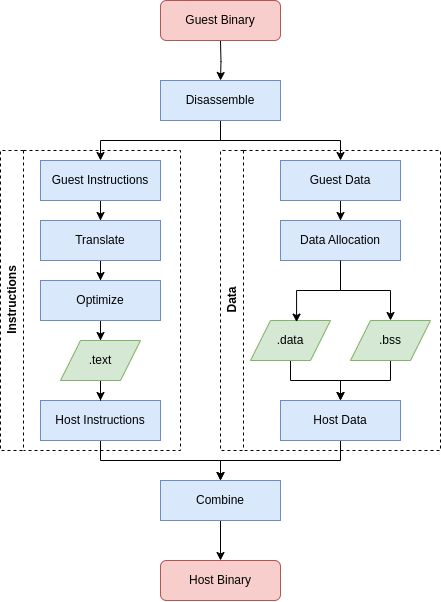
\includegraphics[width=0.6\linewidth]{figures/sta_bin_trans}
    \caption{Static Binary Translation}
    \label{fig:static_binary_translation}
\end{figure}

\subsection{Dynamic Binary Translation}
Dynamic translation is a subset of binary translation.
It involves translating binary code at runtime, as the program executes.
Dynamic translation offers the advantage of adaptability as it can optimize the translation based on the actual execution path of the program, which may vary from run to run.

This method is especially useful in emulating complex software where it's impractical to predict all possible execution paths in advance.
However, it has some drawbacks regarding memory and performance.
When a dynamic translator is running it requires extra space for the program that is being translated.
It needs to allocate space for both the disassembled program and the translated instructions.
This space may balloon very quickly at the start.
The other drawback is the performance penalty of needing to translate instructions before executing them.
This drawback is also mostly evident in the starting phase where the cache is empty.
Overall programs that use dynamic binary translation tend to take up a lot of resources at the start, which decreases after the initial starting phase.

As shown in figure \ref{fig:dynamic_binary_translation} dynamic binary translators have a mechanism against the performance drawback.
They often incorporate a cache to store recently translated instructions, reducing the overhead of re-translating those instructions on subsequent executions. 
This caching mechanism is a key factor in mitigating the performance penalty associated with runtime translation, making dynamic translation an efficient and versatile approach for system emulation and virtualization environments.


\begin{figure}[ht]
    \centering
    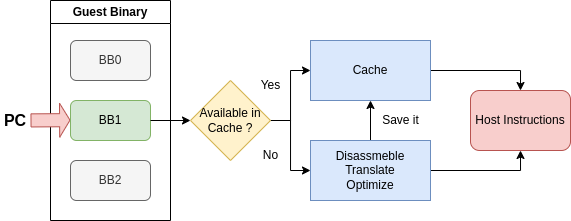
\includegraphics[width=0.8\linewidth]{figures/dyn_bin_trans}
    \caption{Dynamic Binary Translation}
    \label{fig:dynamic_binary_translation}
\end{figure}

\section{Emulators}

Computer emulators are software designed to mimic the hardware of a computer on another.
This allows software designed for the guest system to operate on the host system. 
In this section, we will go into detail about our main targets.
Then we will give a short explanation about the expected output of these emulators which we use for analysis.

\subsection{QEMU}
\ac{QEMU} is a well-known free and open-source emulator and a virtualizer. 
At its core, \ac{QEMU} employs dynamic binary translation which lets the host machine run programs belonging to a different architecture.
Enabling this is the \ac{TCG}, an integral part of \ac{QEMU} that dynamically generates native code for the host CPU.
As shown in figure \ref{fig:qemu_tcg} the \ac{TCG} is used to translate a foreign \ac{ISA} into the host's architecture.

\begin{figure}[ht]
    \centering
    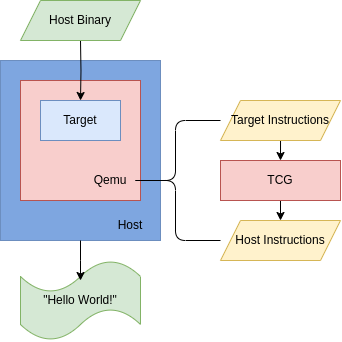
\includegraphics[width=0.7\linewidth]{figures/qemu_TCG2}
    \caption[QEMU translation process]{\ac{QEMU} translation process with \ac{TCG}}
    \label{fig:qemu_tcg}
\end{figure}

\subsubsection{TCG}
\ac{TCG} \cite{qemu_tcg} which began as a generic backend for a C compiler was later improved upon to be both portable and efficient, allowing \ac{QEMU} to quickly translate the guest instructions into a form that can be directly executed by the host machine, thereby improving the speed and efficiency of the emulation process.
This combination of dynamic binary translation and the flexibility of \ac{TCG} enables \ac{QEMU} to provide a high-performance and versatile solution for system emulation.
Thanks to the flexibility of the \ac{TCG}, many different architectures are supported by \ac{QEMU}.

These include \cite{qemu_arch}:
\begin{itemize}
    \item Arm
    \item MIPS (little endian)
    \item PPC
    \item RISC-V
    \item s390x
    \item SPARC
    \item x86
\end{itemize}

\subsection{Arancini}
Arancini is a project from the Systems Research Group at the \ac{TUM}.
It builds on the knowledge gained from two earlier projects: Lasagna \cite{rocha2022lasagne} which translates any x86 program statically to an Arm \ac{ISA} and Risotto \cite{gouicem2022risotto} which emulates x86 program dynamically on an Arm machine.
Like these previous projects, Arancini focuses on making x86 programs work on Arm, but it also adds support for RISC-V systems.
It uses a combination of LLVM, a well-known toolkit for building compilers, and its own custom translation technology to achieve this.

\subsection{Emulator Logs}
An emulator log is a detailed record generated by an emulator during its operation.
They generally capture a wide range of information about the emulator's activities.
For our reproducer to function properly we need to capture specific values either after every instruction or every basic block.
These values include register values and all reads and writes in order.
Generally, emulator logs include more information including the executed instruction, the translated code, and much more.
However, the aforementioned values are enough to know the exact state the binary was in before executing the next step.

\section{Execution Methods}
\subsection{Concrete Execution}
Concrete execution refers to the traditional method of running programs where, the program operates on actual, specific input values to produce outputs.
In this execution model, the program's instructions are carried out step by step, with each operation performed using concrete data values provided at runtime or predefined in the program. 
This method is straightforward and mirrors how programs are executed in real-world scenarios, making it intuitive and easy to understand. 

Concrete execution is particularly useful for debugging, as it allows developers to trace the exact sequence of steps a program takes with a given set of inputs, observing the program's behavior and output directly.
However, its reliance on specific inputs means that concrete execution can only explore one path through the program at a time, limiting its ability to uncover issues that may arise with different inputs or in untested execution paths.

\subsection{Symbolic Execution}
Symbolic execution, on the other hand, abstracts away from concrete input values, instead treating inputs as symbolic variables that can represent multiple possible values simultaneously. 
This approach allows the program to be executed in a way that explores multiple execution paths in a single run, by considering all the possible values that the symbolic variables might take. 
Symbolic execution builds a mathematical model of the program's execution paths, using symbolic expressions to represent the outcome of computations and decisions based on the symbolic inputs. 
As you can see in the figure \ref{fig:sym_tree} every possible branching instruction adds a new path.
\begin{figure}[ht]
    \centering
    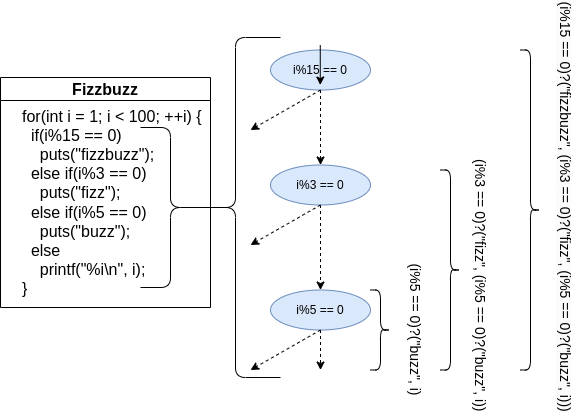
\includegraphics[width=0.8\linewidth]{figures/sym_trans}
    \caption[Branching in symbolic execution]{An example of a branching code in a tree}
    \label{fig:sym_tree}
\end{figure}

This model can then be analyzed to identify potential bugs, security vulnerabilities, or performance issues across a wide range of input conditions without having to enumerate and test each one individually. 
While powerful, symbolic execution is computationally intensive and can face challenges like path explosion, where the number of possible execution paths grows exponentially with the complexity of the program.

\subsection{Concolic Execution} 
Concolic execution, a hybrid approach combining concrete and symbolic execution, aims to mitigate some of the limitations of both methods. 
In concolic execution, the program is run with specific concrete input values, like in concrete execution, but at the same time, it tracks symbolic constraints derived from the execution path taken. 
By analyzing these constraints, concolic execution tools can systematically generate new concrete inputs that will explore different paths through the program, combining the depth of symbolic analysis with the actual values from concrete execution.

This approach allows for more efficient exploration of the program's execution space, making it possible to uncover subtle bugs or vulnerabilities that might not be evident through conventional testing. 
Concolic execution has proven particularly useful in software testing and verification, providing a balance between the thoroughness of symbolic execution and the directness of concrete execution.

\section{Verifier}
In this section, we will go step by step and explore the tools that are used to build the verifier.

\subsection{Theorem Provers}
Theorem provers are computer programs that assist in proving mathematical theorems by formal methods.
The core idea behind theorem proving is to represent mathematical statements and proofs as formal structures that a computer can manipulate.
Theorem provers can then be used to check the validity of these proofs or even to automatically generate proofs for certain propositions within a given set of axioms and rules of inference.

\subsection{Miasm}
Miasm \cite{desclaux2012miasm} is a framework primarily designed for reverse engineering and binary analysis.
It features tools such as a disassembler and a symbolic execution engine.
The framework operates by taking advantage of the features of the symbolic execution engine, where binary code is interpreted in terms of symbolic expressions rather than concrete values.

This symbolic approach allows the theorem solver to evaluate the logical and mathematical properties of the code, solving constraints and proving or disproving theorems about the code's behavior under various conditions.
It also paints a clear picture of the transitions of the register and memory states between instructions and basic blocks.
The produced symbolic expressions are invaluable when comparing different states as they can pinpoint the expected changes and the actual ones.

\subsection{Focaccia}
Focaccia is a specialized verifier program designed to assess the accuracy of emulators.
It uses concolic execution to collect data from a binary and compare it with an emulator's log.
At its core, Focaccia works by comparing these two data sets.
The first set comprises the memory and register values obtained during a test run on actual hardware, which serves as the benchmark or oracle for expected outcomes. 
The second set involves the detailed log produced by the emulator during its operation, which records various actions including register modifications, memory writes, and the current position of the \ac{PC}.
These logs are integral to the verification process as they provide a sequential record of the emulator's behavior, which lets Focaccia find the cutoff point where it starts to behave differently.

The verifier uses the Miasm \cite{desclaux2012miasm} reverse engineering framework for breaking down the original binary code into symbolic expressions for each operational step, transforming the instructions into a more abstract and analyzable form.
These symbolic expressions represent the ideal state changes that should occur step by step according to the software's design.
Then Focaccia does a detailed comparison between these symbolic expressions and the actual state changes recorded in the emulator's log.

This comparison is the focal point of the verifier as it highlights any discrepancies between the expected behavior (as defined by the symbolic expressions) and the actual behavior observed in the emulator.
Discrepancies signal potential bugs in the emulator, indicating that the emulator's reproduction of hardware behavior is not entirely accurate.



% !TeX root = ../main.tex

\chapter{Overview}\label{chapter:overview}

% Overview
% Explain the system overview
% Design goals
% Explain the system workflow
% Identify system components and explain their function


\chapter{Findings}\label{chapter:findings}
In this chapter, we will discuss our findings on bugs related to accelerators and \ac{TCG}.
We will begin by examining the distribution of bugs in \ac{QEMU} to understand the impact of accelerator bugs on development.
Then we will talk a bit about bugs caused by accelerators, followed by a list of bugs found in different accelerator target architectures.
Special attention will be given to x86 architectures as targets.
Additionally, we will delve into bugs that specifically occur on Arm CPUs when running x86 binaries.

Before we start, it is important to note that this survey is based on data from \ac{QEMU}'s GitLab repository \cite{qemu_issues}.
As of this writing, there are a total of 2140 issues, with the oldest one dating back to 2021.
Some bugs have been transferred from the previous repository, making it challenging to determine their exact date.
Figure \ref{fig:issues} shows the distribution of relevant bugs for reference.

\begin{figure}[ht]
    \centering
    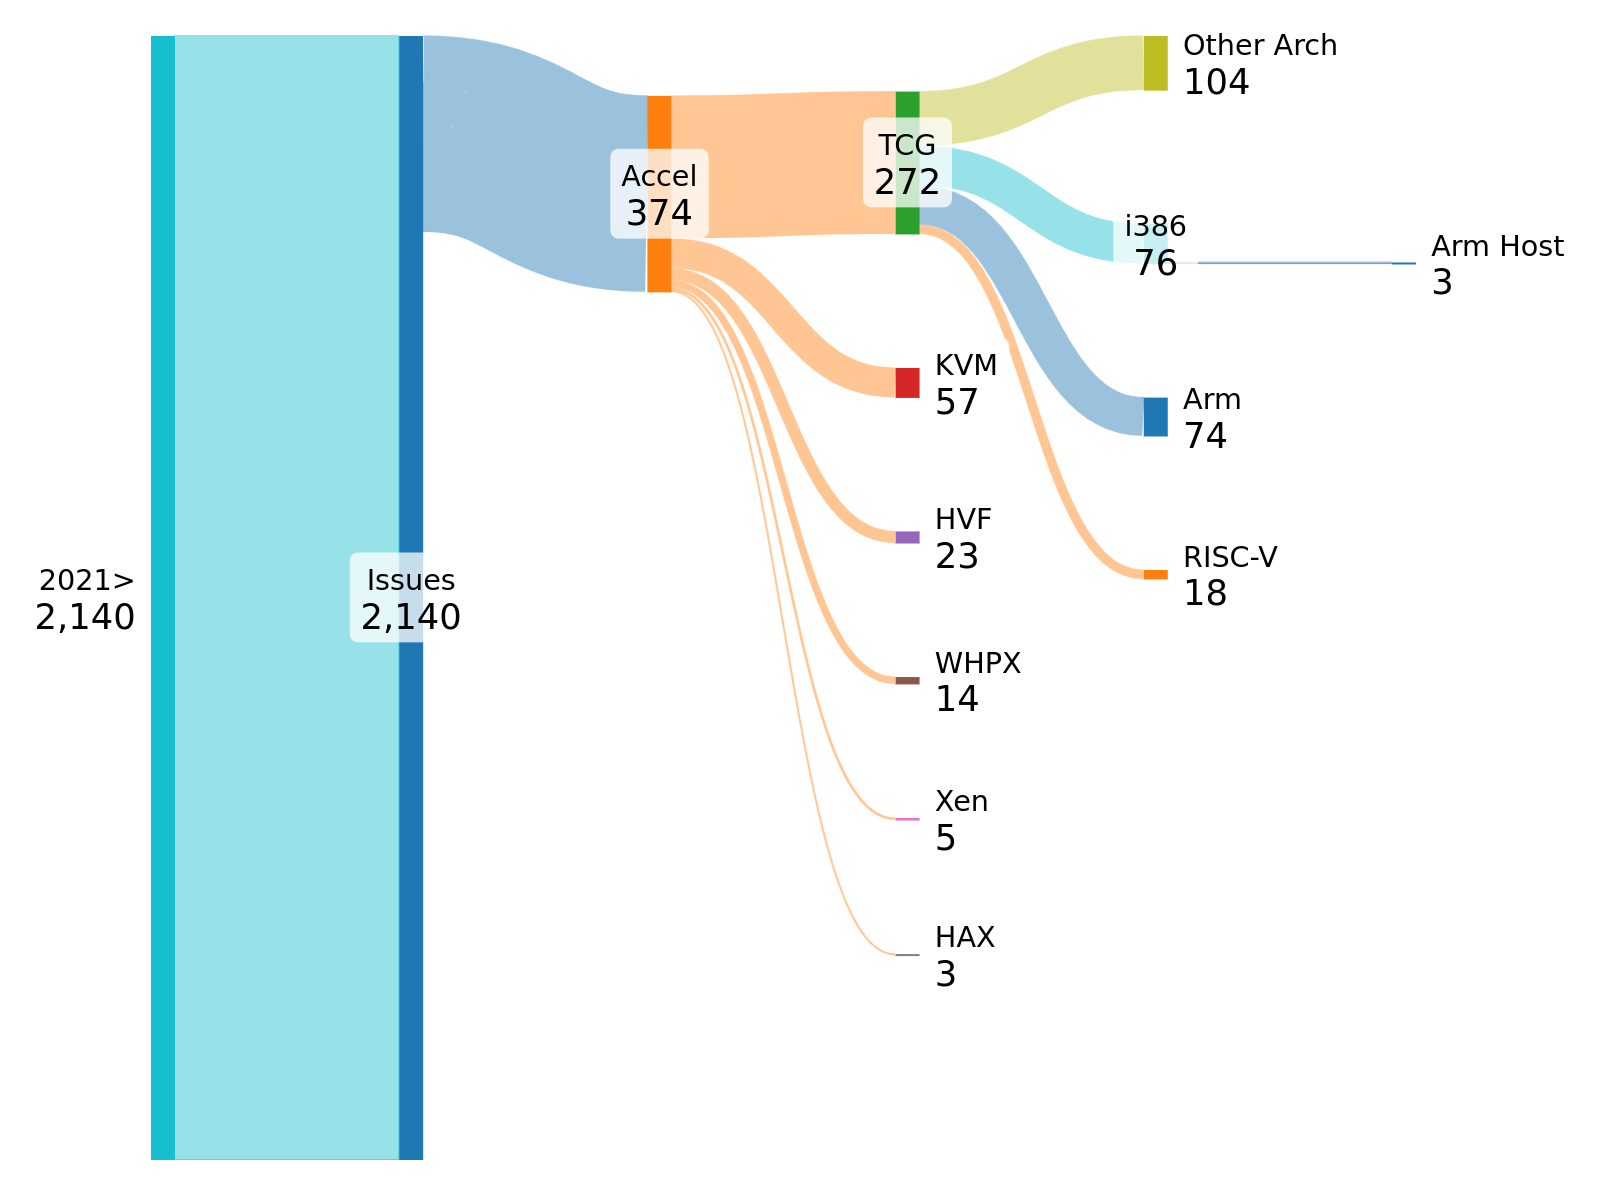
\includegraphics[width=0.8\linewidth]{figures/issues3}
    \caption[QEMU bug distribution]{Sankey diagram showing the distribution of relevant issues}
    \label{fig:issues}
\end{figure}

\section{Distribution of Bugs in \ac{QEMU}}
As is visible in figure \ref{fig:issues} \ac{QEMU} has more than 2000 bugs.
The current version of \ac{QEMU} has 2038147 \ac{sloc} split between different programming and scripting languages according to the line counting program cloc \cite{cloc}.
Drawing from Steve McConnell's research on software metrics \cite{sloc}, we can compare \ac{QEMU}'s bug frequency to that of commercially released products, indicating that \ac{QEMU} has a relatively clean codebase.

Out of all the bugs, 374 are related to accelerators, accounting for about 15\% of the total.
This suggests that the accelerator-related issues are a significant part of the total amount of bugs.
Among these accelerator bugs, the majority, or about 70\%, stem from \ac{TCG}, which is expected given that \ac{TCG} is the primary and most widely used accelerator.
KVM related bugs make up another 15\%, with the remaining 15\% spread across other accelerators.

Regarding \ac{TCG} specific bugs, those involving x86 (i386) and Arm architectures are the most common, each being roughly around 30\% of the total.
This should not come as a surprise since these architectures are being utilized most commonly, leading to extensive usage and testing.

\section{x86 Translation Errors}
In this section, we will go over the bugs encountered when running x86 binaries using the \ac{TCG}.
Most of these bugs are host architecture and operating system independent and tend to arise from incorrect implementation of individual instructions.

We've organized these bugs into six categories based on how they affect the emulation:
\begin{itemize}
    \item Calculation Error: These are mistakes in instructions that either lead to incorrect calculations or issues with flag registers either being incorrectly set or not set at all. However, they don't usually interrupt the flow of the program.
    \item Exceptions: These bugs trigger an exception in \ac{QEMU}, causing the emulation to stop abruptly.
    \item Errors: Similar to exceptions, these issues cause \ac{QEMU} to halt the emulation process.
    \item Segmentation Faults: These occur when the program attempts to access memory areas it doesn't have permission to. While this doesn't happen on actual hardware, it is somehow triggered during the emulation.
    \item Hardware Problems: These bugs impact external hardware, potentially making it unusable or significantly less efficient.
    \item Other Bugs: This category includes bugs that don't fit into the other groups, either because their origin is unclear or because they were introduced in newer versions by mistake.
\end{itemize}

The results of the survey are expressed in the table \ref{tab:tcg_x86}.
In the next sections, we will mainly focus on calculation errors, since this is where the verifier shines the most.
It would be challenging to test the other bugs since they don't necessarily finish their execution normally, therefore leaving the emulator logs incomplete.

\begin{table}[htpb]
    \caption[x86 TCG error distribution]{Distribution of TCG errors for x86.}\label{tab:tcg_x86}
    \centering
    \begin{tabular}{l r r r}
      \toprule
        Type & Number & Closed & Open \\
      \midrule
        Calculation Error & 18 & 12 & 6 \\
        Exceptions & 6 & 4 & 2 \\
        Errors & 3 & 2 & 1 \\
        Segmentation Faults & 14 & 10 & 4 \\
        Hardware Problems & 1 & 0 & 1 \\
        Other & 33 & 26 & 7 \\
      \bottomrule
    \end{tabular}
\end{table}

\subsection{Interpretation and Evaluation of the Bug Survey}

\paragraph{Other:}
As is visible in table \ref{tab:tcg_x86} most errors that originate from x86 emulation belong to this category.
And these errors, make up nearly 45\% of the total amount.
Unfortunately, the bugs that cause these problems are multiple and complex therefore they cannot be easily traced to simple instructions.
Depending on the complexity the verifier can find the bug and the reproducer might be able to reproduce it.
However, it is more than likely that the steps that result in these bugs cannot be simply repeated to pinpoint the actual reason.
Therefore it is quite difficult to reproduce them, making our project a bad match against them.

\paragraph{Hardware Problems:}
There's only a single reported hardware problem, and due to limited information, it's hard to analyze it.
Considering that it is a hardware problem errors of this kind are more likely to be a part of the IO and have nothing to do with emulated instructions.

\paragraph{Segmentation Faults:}
These types of bugs are another frequent issue, accounting for nearly 20\% of all bugs.
A \ac{segfault} happens when a program attempts to access a nonexistent or restricted area.
These accesses can be classified into three categories:
\begin{itemize}
  \item Read
  \item Write
  \item Execute
\end{itemize}
Generally, the best way to solve these bugs is to trace them and find the location where they caused the \ac{segfault}.
In most cases an emulator will keep running and outputting the emulator log until one of the aforementioned events happens.
After the \ac{segfault} happens the the program will be stopped abruptly and the emulator will stop.
This means the emulator log will be stopped before reaching the end.
Even though in the case of a segmentation fault the emulator trace will be cut off, considering that we only need to find the address where this happens along with the used instructions the verifier can be helpful.

Although the verifier can prepare the snapshot and the symbolic expression, the current version only finds errors by comparing states.
This means it will stop before noticing that the emulator log is short.
Theoretically, if the \ac{segfault} is happening because of an instruction the reproducer should be able to reproduce it. 
However, in most cases, this is not possible since the reproducer ignores some details.
A \ac{segfault} happens for multiple reasons, either because the memory location doesn't have the required permissions or because it doesn't exist at all.
However, neither the verifier nor its symbolic log has any knowledge about a memory location's permissions.
Therefore even if we can extract the offending instruction and the used values, without being able to set the memory location's permissions we cannot set an equivalent environment.

In this case, we have two choices.
We can handle it just like other memory access instructions where we allocate space on the data section and then use it for reading or writing.
Or we can keep the original address.
In the first case, we are very likely to not trigger the fault since we use the location that we have declared and made sure it exists.
In the second case, we have no idea whether this original address exists and what its value and permissions are.
Therefore this method would cause undefined behaviour.
Because of these reasons, the reproducer is not a good match for this type of error.
The best we can expect to do is to try the first way and see whether we can trigger the \ac{segfault} consistently.

\paragraph{Errors and Exceptions:}
Errors and exceptions are relatively common in \ac{QEMU}, leading to the program stopping. These issues likely stem from the emulator's internal state, suggesting that alternative debugging methods might be more effective.

\paragraph{Calculation Errors:}
Finally, we have the calculation errors.
They make up slightly less than 25\% of total errors, but they are theoretically the most challenging to detect as they involve instructions behaving slightly differently than expected.
For example, some instructions might set a bit to a wrong value or change another bit that it shouldn't touch.

The main problem with these instructions is that these values are not necessarily used.
This means these programs can go a long way before exhibiting the bug since the difference might have happened multiple instructions ago.
Or maybe the result is close enough to the expected answer and therefore it is not found out.

However, in a good case, this instruction just calculates wrong values, and this discrepancy is detected.
Our verifier and reproducer combination is a good match for these instructions since it uses symbolic execution we can catch every detail and compare it with the emulator log.

\subsection{Detailed Inspection of Bugs on Arm}
In the following subsections, we will go over specific bugs that only appear on Arm devices.
We are inspecting these bugs extra thoroughly because we are interested in seeing whether some bugs appear depending on the host hardware.
Out of 76 bugs that we have seen so far, only 3 of them are Arm specific.
Considering this fact, we can assume that hardware-specific bugs are rather rare.
After taking a closer look at the following subsections, it should be clear that these bugs are not because of the host architecture but because of other reasons.

\subsubsection{Issue \#1659}
The first issue specific to Arm was discovered in an aarch64 system running Darwin.
This bug caused the emulator to freeze and enter a continuous shutdown loop.
It was traced back to the floatx80\_div instruction.
Upon closer examination, it was determined that the problem was due to a miscompilation by Clang.

Therefore, this issue is not directly related to the emulator itself but to the compiler, meaning we can cross this issue from the Arm only list.

\subsubsection{Issue \#2101}
The second issue was identified on a system using Fedora Linux as the host.
This bug manifests itself when executing the ls command within \ac{QEMU}.
It results in incorrect output that omits several directories.
Due to the lack of more information, it is not possible to find the actual cause.

\subsubsection{Issue \#2168}
The final issue also happens in Linux.
This time when running grep on Gentoo Linux inside \ac{QEMU}, a segmentation fault occurs.
Similar to the previous issue, there is limited information available, making it difficult to provide more insights.




% !TeX root = ../main.tex

% Design
% Explain the system design in detail
% Explain each system component sufficient details
% Explain workflows using algorithms
\chapter{Design}\label{chapter:design}
The following chapter presents the core design decisions that were taken to extend the Focaccia verifier with the reproducer.
Extra attention is given to the reproducer interface, the data taken from the verifier, and how it relates to the whole reproducer.
After a brief look at the interface, we will explore the reproducer and discuss in more detail how we create the environment for the reproduced program.
This step will go over the instructions we are trying to reproduce, along with setting up the registers, memory, and stack.

\section{Focaccia Interface}
The reproducer, which was designed as an add-on, comes after the verification process is done.
The verification process's output is a long list of calculations that occur at every step of the program's execution.

The result of these calculations is the following:
\begin{itemize}
    \item pc: The program counter can be used as a pseudo key that maps the calculations to the instruction or the basic block it belongs to. However, it is not a unique key since the same block can be repeated multiple times.
    \item snap: The snapshots are the concrete values that have been extracted. These include both register values and memory values.
    \item txl: This is the difference between the current snapshot and the next one. This difference only includes registers.
    \item ref: These are the reference changes that happen during the execution of the instruction or the basic block. They are in the form of symbolic expressions and play a vital role when creating the reproducer program.
    \item errors: This is a list of errors found while comparing the emulator log with the symbolic execution. There are multiple levels of errors depending on their severity.
\end{itemize}

Of the five entries mentioned, only two are essential for the reproducer, and an additional one is useful but not mandatory.
Another entry is used to identify bugs, whereas the final entry is not used at all.

\paragraph{errors:}
The verification process generates five different types of outputs, with errors being one of the key outputs.
They are used to filter through the output list to find exactly which steps have problems in them.
They are not necessarily used in the reproducer, but rather, they are used to pinpoint the places where the reproducer should be used.

\paragraph{snap:}
The snapshot is one of the three inputs that the reproducer takes.
They are called snapshots because they represent the exact state of the CPU just before the instruction is executed.
They include not only the used values but also all of the register values and all of the memory values, which results in a lot of irrelevant information.
We need a way to filter them in order to extract only the necessary values used in our setup.
This filtering step can be done by using symbolic expressions. 

\paragraph{txl:}
The next output, txl, does not directly contribute to the reproducer.
Since this output only shows the differences between the current and the following snapshot, it does not give any hints about the instructions.
Neither does it help find values that belong to the previous state of the execution process.
Therefore these values are not used in the reproducer.

\paragraph{pc:}
This entry is the program counter, and it is used to check whether the symbolic expression aligns with the snapshot.
We can use it this way since it is supposed to have the same value as the RIP register in x86.
Previously, we used it to find the location of the basic block that was turned into a symbolic expression.
However, updates to the verifier have made this step redundant since we can now directly convert symbolic expressions back into assembly instructions.

\paragraph{ref:}
The final output is the ref, a symbolic expression representing the changes our snapshots undergo when we execute the next instruction.
These symbolic expressions have multiple purposes.
Firstly, they can be used to extract the assembly instructions needed for our program.
As mentioned before, we used to use the PC to extract the basic block, but with updates to the verifier, it became able to pinpoint the problematic instructions instead of the whole basic block.
This meant that extracting the instructions used would be difficult without getting the proper cutoff point.
Instead of trying to guess the actual point, the symbolic expression is used to get the exact instructions.

Secondly, the symbolic expression can be filtered to identify which registers are used for which cases.
These registers can be later matched with the correct values using the snapshots.
However, there is a special case where this is more complex.
If the registers are used to address something in the memory, we cannot directly use the same addresses since these addresses would point to memory locations with uninitialized data.
Instead, we need to allocate data somewhere else and put its address into these registers.

\section{Design of the Reproducer}
In this section, we will go over the design of the reproducer.
Since we have already explained the verifier's outputs and how they relate to the reproducer, we will mainly concentrate on the different parts of the reproducer.
The inner workings of the reproducer are depicted in figure \ref{fig:reproducer} in order to provide a clear picture of the data flow.
The creation process of the data section is shown in figure \ref{fig:data} while figure \ref{fig:text} shows the text section.

\begin{figure}[ht]
    \centering
    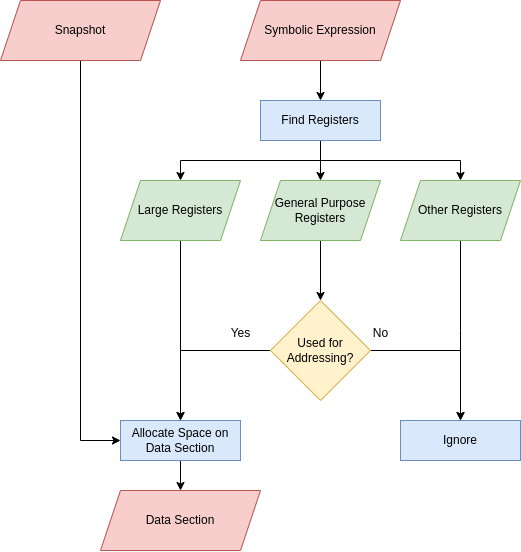
\includegraphics[width=0.8\linewidth]{figures/data}
    \caption{Process of creating the data section.}
    \label{fig:data}
\end{figure}

\begin{figure}[ht]
    \centering
    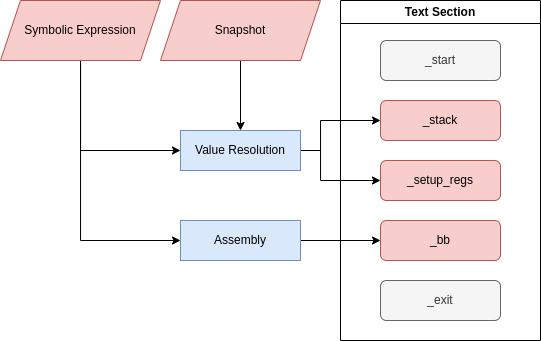
\includegraphics[width=0.8\linewidth]{figures/text}
    \caption{Process of creating the text section.}
    \label{fig:text}
\end{figure}

\subsection{Instructions and Basic Blocks}
The verifier is designed to reproduce bugs that come up in bigger programs.
This process entails finding the exact instruction that triggers a bug and then recreating a similar situation.
In our case, as depicted in the figure \ref{fig:text} this instruction is supplied by the symbolic expression and directly appended to the text section.
No adjustment is needed, so we append it without any change.

However, there is a slight problem in handling instructions that way.
This way of reproducing the bugs only lets us handle calculations.
If we tried the same thing with other instructions that changed the program flow, we would jump to unknown places with unknown consequences.
The same goes for instructions that affect hardware.
These special cases are handled in the following section.

\subsection{Registers}
Setting up registers according to their original values is also essential for the reproducer.
Some bugs might only be triggered when the registers are filled with particular values.
To set the correct environment, we have to handle these values correctly.
Registers are used for two primary purposes.

Firstly, they are set with values that are independent of the state of the emulator and the memory layout.
For instance, a register storing value 5 for a mathematical calculation fits this description.
For such registers, we don't need to transform their value; we can directly set them with the same value.
The second case involves registers that depend numerically on a memory address, requiring additional handling, given that we have not explicitly allocated any memory yet.
Handling these registers is done in both the data and text sections.
Figure \ref{fig:data} shows where they are used in the data section, and figure \ref{fig:text} depicts the register setup in the code section.

The values of registers can be split into three categories as shown in figure \ref{fig:data}.
These categories are:
\begin{itemize}
    \item Large register values
    \item Address
    \item Other register values
\end{itemize}
All of these categories have different calculation methods, with some being relatively straightforward and others needing multiple calculations where we leverage symbolic values for resolution.
In the following paragraphs, we will go into more detail about how they are calculated.

\paragraph{Large register values:}
Large register is the common name we have given to any register that cannot be filled directly with immediate values.
In these cases, even though we can easily extract the value from the snapshot, we cannot put them into assembly instructions.
Instead, we have to save the actual value in the memory as a constant and then use a special move instruction with the constant value's address to move it to the register.

We handle these in two steps.
In the first step, we save these register values to the data section.
Then, when we write the values into the registers, we use the aforementioned special move instructions with the addresses.
This way, we can set these large registers.

\paragraph{Addreses:}
These values are generally inside the 64-bit general-purpose registers.
The assembly instructions use them for read or write operations.
Unlike the other types of instructions, we cannot simply copy them because they point to memory locations that only exist for the original program.
Instead, we need to allocate space in the data section and then change every address pointing to the original one with the new one.

When doing this, we need to take care of a couple of details.
Firstly, we can both read and write in the same memory location.
In this case, we need to be aware that this address is used in multiple places and not create a new one.

The second case concerns the readable and writeable chunk sizes and how they align.
We might need to read and write to a continuous memory chunk.
However, the data from the symbolic expression might point to a random order of reads and writes that do not even align with the size.
In this case, we might order these addresses, but the size of the reads and writes might cause confusion.
To prevent problems from arising, we split all of these memory locations into bytes.
This means we always have an address for any byte that is read or written to.
In figure \ref{fig:addr_match}, we can see a comparison of the naive approach and our approach.

\begin{figure}[ht]
    \centering
    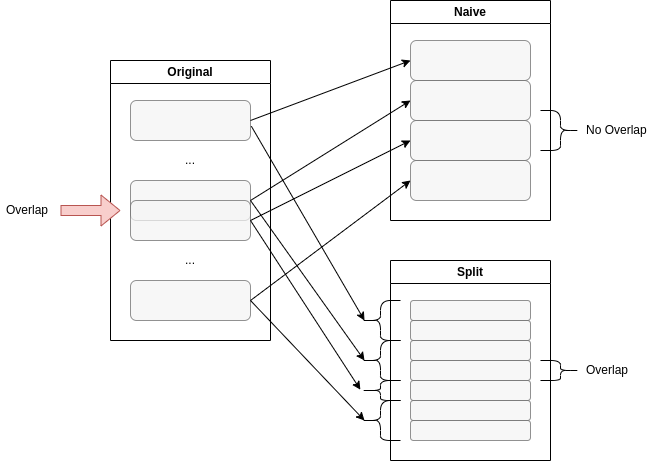
\includegraphics[width=0.8\linewidth]{figures/alloc2}
    \caption{Naive approach to data allocation versus our strategy.}
    \label{fig:addr_match}
\end{figure}

\paragraph{Other register values for calculation:}
Finally, we have all of the other registers.
These registers can be set by immediate values.
This makes setting them up relatively easy since we just need to read the values from the snapshot and use the correct move instruction according to their type. 

\subsection{Memory}
In the last subsection, we have an overview about using addresses but the actual method of finding these addresses is more complicated.
We can gather three subsets of symbolic information from the one we have been given. These are:
\begin{itemize}
    \item Used memory addresses
    \item Changed memory addresses
    \item Used registers
\end{itemize}

By using the first two items, we can find which values are used to address memory.
However, these would be just the addresses and not the actual values of the registers.
In x86, an address can be made out of base, index, scale, and displacement.
Out of these four parts, the first two are registers, and the latter are constants.
Only the base is necessary, while the other ones can be omitted.
This means there are multiple ways an address's symbolic expression can look, but they all include the base register.

Although we can write a program that can evaluate every possible base, index, scale, and displacement combination, there is a better way.
We can separate the offset from the base by evaluating the base register and the whole address.
When we prepare the new address, we can subtract this offset from the displacement.
This will allow us to ignore the original offset when running the code since we have already subtracted the offset, which will later be added.
This calculation is depicted in figure \ref{fig:mem_addr}.
Using this method, we can keep the original values for everything except the base and do not need to consider how the addressing is made.

\begin{figure}[ht]
    \centering
    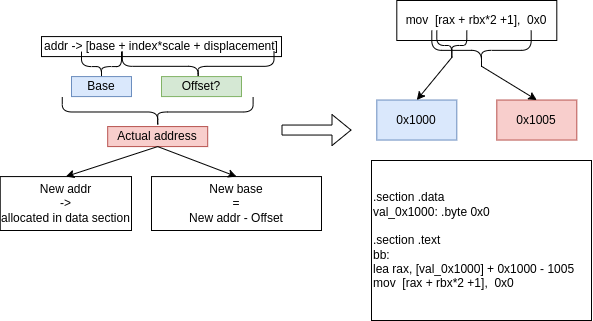
\includegraphics[width=0.9\linewidth]{figures/mem_addr}
    \caption{Calculating the new effective address using the offset and the allocated address.}
    \label{fig:mem_addr}
\end{figure}

\subsection{Stack}
Setting the stack state is the final step in configuring the reproducer.
This step is not required for every instruction but is essential for operations that involve the stack, such as push, pop, or any memory addressing that relies on the stack pointer.
The method for finding the values in the stack is the same as the memory values; we evaluate expressions related to memory reads or writes.
However, we pay special attention to whether these symbolic expressions involve the stack pointer.

Although the approach for identifying stack values mirrors that used for general memory operations, initializing these stack values demands a different method.
Unlike other memory operations where the exact location is flexible as long as there is enough space and the registers have the correct addresses, the values in the stack need to be in the correct positions.
Therefore, the values related to the original stack must maintain their relative positions relative to the stack pointer.

We first need to gather the correct values to reconstruct the stack.
Generally, not all of the values on the stack are used for the instructions given.
Therefore, we cannot recognize them.
In that case, we substitute these values with zeros.
When collecting these values and adding the padding, it is essential to remember that the values are not only before (in higher addresses) the stack pointer but also after (in lower addresses) it.
This means we need to put all the values into the stack and then ensure that the stack pointer is in the correct place.
We do this by pushing all the values to the stack and subtracting the number of bytes whose addresses are smaller than the original stack pointer from the new stack pointer.
By using this method, we recreated the stack.

\begin{figure}[ht]
    \centering
    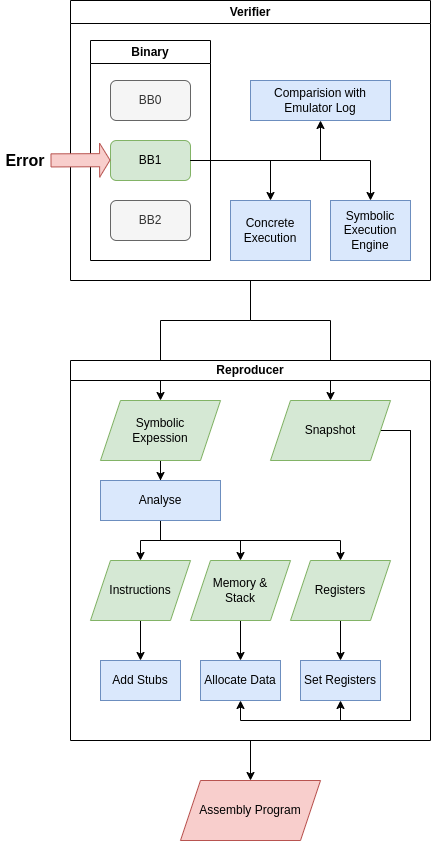
\includegraphics[width=0.6\linewidth]{figures/rep}
    \caption{Overview of the Reproducer.}
    \label{fig:reproducer}
\end{figure}

% !TeX root = ../main.tex

% Implementation
% Explain all low-level implementation level details
\chapter{Implementation}\label{chapter:implementation}
This chapter will review low-level implementation details and explain what we had to do to get the reproducer working.
Firstly, we will talk about our additions to the verifier.
Then, we will discuss our Python program and explain the functionality of the two classes we designed.
Finally, we will review cases where the verifier might not work as expected.

\section{Additions to the Focaccia}
Focaccia is a full-fledged verifier that can be used to find bugs in emulators that stem from the wrong implementation of instructions.
However, because it was designed as a verifier, it lacks some useful features that would have helped the reproducer.
In this chapter, we will go over our additions to amend this.

Firstly, the original verifier would not return the actual state of the program before the execution of an instruction.
Naturally, this made it quite challenging to know what was inside the memory and registers.
We patched the verifier to return the snapshot of the program.

Our second addition was to the symbolic execution part of the verifier.
The symbolic expressions that the verifier can isolate are quite helpful.
It can return the following values from a given symbolic expression:
\begin{itemize}
    \item Symbolic expressions of the used and changed memory addresses
    \item A list of used registers
\end{itemize}
Both of these outputs are helpful since we can see which registers need to be restored and which memory locations need which values.
If we could change anything without considering the underlying hardware mechanisms like paging, permissions, and the actual location of the program in the memory, this might have been enough.
However, since this is not possible within this project's scope, we decided to allocate space in the data section and use it for memory.
This meant we needed to find the registers used explicitly for addressing the memory and change their values to point to the addresses in the data section.

We made this by adding a function to the symbolic execution program to evaluate any given expression except a register.
This meant that given a symbolic expression that points to an address, we could extract the used registers.
Then, we can be sure that these registers address memory and handle them as such.

The same mechanism also works for the stack.
We filter the symbolic expressions that point to memory for the stack pointer and assess whether they were used in the stack.

\section{Python Classes}
Since we were extending the verifier, we used the same programming language it was implemented in, namely Python.
Our reproducer is made up of two classes.
The first one, which is target agnostic, is called ReproducerEntry.
This class extracts information from the snapshot and the symbolic expressions.
The second class is called x86Reproducer.
As the name suggests, this class is x86 architecture-specific and is tasked with producing assembly instructions for its architecture.
The flow of data can be seen in figure \ref{fig:rep_ent}.
As the figure suggests, ReproducerEntry splits the snapshot using the symbolic expression and sets the x86Reproducer with the necessary values.
After this, the x86Reproducer prints the assembly code.

\begin{figure}[ht]
    \centering
    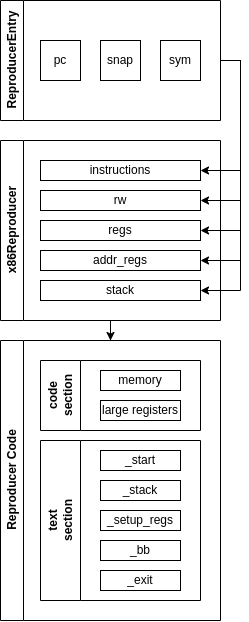
\includegraphics[width=0.5\linewidth]{figures/rep_ent}
    \caption{Flow of the reproducer including the ReproducerEntry and x86Reproducer classes.}
    \label{fig:rep_ent}
\end{figure}

\subsection{ReproducerEntry}
The backbone of our reproducer is the ReproducerEntry class.
It lets us find all of the necessary data using the snapshot and the symbolic expressions.
The main functionality of this class is shown in figure \ref{fig:rep_ent}, but we will go over the details:

\begin{itemize}
    \item get\_instructions:
    This function returns a list of instructions that make up the erroneous basic block.
    These instructions are received from only the symbolic expression.
    \item get\_rw\_addr:
    This function returns a dictionary of reads that will happen during the execution of the basic block and the writes that will happen as a result.
    Each entry is for a single byte; its key is the address.
    The reads keep the original values, while the writes are initialized with zeros.
    \item get\_regs:
    This function returns the dictionary of registers that are needed for the execution of the basic block.
    \item get\_addr\_regs:
    This function also returns a dictionary of registers.
    However, these are dictionaries that were only used for addressing memory.
    Moreover, the values of these dictionaries are not the register's values but the actual address they were used to point to.
    \item get\_stack:
    This function returns two values.
    Firstly, it returns the number of bytes that were subtracted from the stack pointer (either due to push operations or just subtraction from the stack pointer).
    Secondly, it returns the values that were in the stack.
    If a particular value is unused, its place is filled with zeros.
\end{itemize}

As shown, the ReproducerEntry is a versatile class that can extract everything we need from the snapshot and the symbolic expression.

\subsection{x86Reproducer}
This class is the part that produces the assembly instructions.
It is specifically designed to produce x86 assembly.
It receives all the information from the ReproducerEntry and does not directly use the snapshot or the symbolic expression.

In the data section, we initialize the values using the register and read/write dictionaries.
In the text section, the basic block is combined with stack and register setup code along with start and exit stubs.
The stack setup only uses what was returned from the stack values, while the register setup uses both the regular register dictionary and the addresses register dictionary.

\section{Shortcomings}
When trying to understand the reproducer's shortcomings, it is essential to remember that it was designed as an add-on to the verifier, which in turn depends on Miasm to work correctly.
As mentioned, our reproducer has some shortcomings regarding special registers and instructions.
This section will review these cases and explain why they are difficult to deal with.

Two crucial points should be considered when explaining why it is not possible to replicate bugs perfectly.
First of all, computer programs run step by step.
Each step changes the program's state, writes values to memory, and changes registers.
However, these are not all of the changes.
When a program is running, stack frames are built or destroyed, new pages are added, permissions are updated, and data handled by the kernel are changed.

A program is more than just its address space.
When trying to understand bugs that stem from emulation, we need to keep in mind that the hardware in the background is also part of the program.
All of the aforementioned data must be changed to replicate the state perfectly.
The simplest method to set the state is to run the program until that exact point is reached.


The second point is the symbolic expressions.
They are good at showing state transitions and building a tree for the execution path.
Nevertheless, they are an abstraction and lack details that might point to the bugs.
They do show what instructions do, but they are all on a transactional level.
For example, a symbolic expression might show a read operation, but it does not necessarily show whether the read address was an IO port or it was on a page that did not exist.
Therefore, we use it to guide us in the best way we can.

\subsection{Shortcomings of the Reproducer}
The reproducer has managed to reproduce bugs and code snippets that generally use simpler instructions to do calculations.
However, there are some shortcomings regarding more complicated instructions that affect the program flow or some registers for controlling the hardware.
These limitations will be discussed in the following sections.

\subsubsection{Instruction Pointer}
In CPUs, the instruction pointer is used to select the next instruction which will be executed.
Normally each instruction increments it by that instruction's size.
However, some instructions like jump, call, and return change the instruction pointer arbitrarily.
When this happens, the program expects its execution to continue somewhere else.
In these cases, the execution path changes to a different location, making testing them difficult.

\subsubsection{Segment Registers}
These registers were designed to let the original x86 CPU address more than 64 KB of memory.
However, these are currently used for other purposes like thread-local storage and canary-based stack protection.
Since changing them is very error-prone and these types of registers do not target the class of bugs we are trying to replicate, we decided to ignore them.

\subsubsection{Return Address}
When building the stack for the erroneous basic block,  the stack was set by using the values directly from the original snapshot.
We push these values directly after the start section.
However, this means that the return address of the function is wrong.
It is either zero, if it is not used at all, or it is the original return address.
Both of these values are likely to crash the program if used to return from the start section, but since we directly use the exit system call, the return address has no effect on the program.

\subsubsection{Indirect Memory Access}
Although our program can find memory access using reads and writes, we only look for them in the registers.
This makes sense since we must use at least one register to address a memory location.
However, in cases where a memory location has a pointer to a different address, our program cannot recognize them, and it will copy the same value, meaning it would be pointing to an unknown location.

This cannot happen when the reproducer is used for a single instruction since the address must already be in the register.
If a basic block is used and this problem arises, the best way to deal with it is to run the reproducer on every single instruction.
This method should prevent bugs arising from indirect memory access in a single basic block. 

\subsection{Segmentation Faults}
As we have mentioned previously, the verifier cannot detect \ac{segfault}s because, without the state that comes after the \ac{segfault}, the verifier will fail.
Even though the previous state is enough to set the reproducer, it will not be detected therefore it cannot recreate the bugs.

This weakness can be solved by adding a \ac{segfault} error to the verifier that happens when the emulator log is shorter than expected.
In that case, the reproducer can theoretically produce a program that can trigger the same \ac{segfault}.

However, this is not as simple as it sounds.
This might not always work because some \ac{segfault}s happen on special cases like alignment of the data or permissions of the memory section.
Unfortunately, the reproducer is oblivious to these things, making it difficult to replicate them.

\subsection{Shortcomings of the Symbolic Execution Engine}
We have added this section here to mention that our project relies on the verifier to function, which in turn relies on the symbolic execution engine.
This means that if the symbolic execution engine has problems like unimplemented instructions, our reproducer also suffers.

We have tested our reproducer with many different programs and noticed that most instructions that should have caused the bugs were not implemented in Miasm.
This had multiple different effects on the reproducer.
Sometimes, instructions would be mistranslated, and sometimes, they would be missing.
There is no simple solution except to fix Miasm itself.

% !TeX root = ../main.tex

% Evaluation
% Explain the high-level research questions
% Experimental testbed, benchmarks, methodology
% Evaluate the research questions/hypotheses
\chapter{Evaluation}\label{chapter:evaluation}



talk about the error types 
and if we have recreated an error
maybe test all errors from last two years
a survey about the bugs

maybe talk about hte change
% !TeX root = ../main.tex

% Related Work
% Organize the related work in major categories
% First explain all related work in sufficient detail
% Also, explain how the related work compares to your own work
\chapter{Related Work}\label{chapter:related_work}




% !TeX root = ../main.tex

% Summary and Conclusion
% First summarize the overall work
% Explain the key findings and impact
% Mention the source code
\chapter{Summary and Conclusion}\label{chapter:summary_and_conclusion}



Extend focaccia
make debugging emulators easier
% !TeX root = ../main.tex

\chapter{Future Work}\label{chapter:future_work}
fuzzing?
% Future Work
% Explain the future work

% !TeX root = ../main.tex
% Add the above to each chapter to make compiling the PDF easier in some editors.

\chapter{Introduction}\label{chapter:example}

\section{Section}
Citation test~\parencite{latex}.

Acronyms must be added in \texttt{main.tex} and are referenced using macros. The first occurrence is automatically replaced with the long version of the acronym, while all subsequent usages use the abbreviation.

E.g. \texttt{\textbackslash ac\{TUM\}, \textbackslash ac\{TUM\}} $\Rightarrow$ \ac{TUM}, \ac{TUM}

For more details, see the documentation of the \texttt{acronym} package\footnote{\url{https://ctan.org/pkg/acronym}}.
\subsection{Subsection}

See~\autoref{tab:sample}, \autoref{fig:sample-drawing}, \autoref{fig:sample-plot}, \autoref{fig:sample-listing}.

\begin{table}[htpb]
  \caption[Example table]{An example for a simple table.}\label{tab:sample}
  \centering
  \begin{tabular}{l l l l}
    \toprule
      A & B & C & D \\
    \midrule
      1 & 2 & 1 & 2 \\
      2 & 3 & 2 & 3 \\
    \bottomrule
  \end{tabular}
\end{table}

\begin{figure}[htpb]
  \centering
  % This should probably go into a file in figures/
  \begin{tikzpicture}[node distance=3cm]
    \node (R0) {$R_1$};
    \node (R1) [right of=R0] {$R_2$};
    \node (R2) [below of=R1] {$R_4$};
    \node (R3) [below of=R0] {$R_3$};
    \node (R4) [right of=R1] {$R_5$};

    \path[every node]
      (R0) edge (R1)
      (R0) edge (R3)
      (R3) edge (R2)
      (R2) edge (R1)
      (R1) edge (R4);
  \end{tikzpicture}
  \caption[Example drawing]{An example for a simple drawing.}\label{fig:sample-drawing}
\end{figure}

\begin{figure}[htpb]
  \centering

  \pgfplotstableset{col sep=&, row sep=\\}
  % This should probably go into a file in data/
  \pgfplotstableread{
    a & b    \\
    1 & 1000 \\
    2 & 1500 \\
    3 & 1600 \\
  }\exampleA
  \pgfplotstableread{
    a & b    \\
    1 & 1200 \\
    2 & 800 \\
    3 & 1400 \\
  }\exampleB
  % This should probably go into a file in figures/
  \begin{tikzpicture}
    \begin{axis}[
        ymin=0,
        legend style={legend pos=south east},
        grid,
        thick,
        ylabel=Y,
        xlabel=X
      ]
      \addplot table[x=a, y=b]{\exampleA};
      \addlegendentry{Example A};
      \addplot table[x=a, y=b]{\exampleB};
      \addlegendentry{Example B};
    \end{axis}
  \end{tikzpicture}
  \caption[Example plot]{An example for a simple plot.}\label{fig:sample-plot}
\end{figure}

\begin{figure}[htpb]
  \centering
  \begin{tabular}{c}
  \begin{lstlisting}[language=SQL]
    SELECT * FROM tbl WHERE tbl.str = "str"
  \end{lstlisting}
  \end{tabular}
  \caption[Example listing]{An example for a source code listing.}\label{fig:sample-listing}
\end{figure}

% TODO: add more chapters here

\appendix{}

\microtypesetup{protrusion=false}

\addchap{Abbreviations}
\begin{acronym}
	\itemsep-.25\baselineskip
	\acro{TUM}[TUM]{Technical University of Munich}
	\acro{TCG}[TCG]{Tiny Code Generator}
	\acro{PC}[PC]{Program Counter}
	\acro{clib}[clib]{C Standard Library}
	\acro{TCG}[TCG]{Tiny Code Generator}
	\acro{QEMU}[QEMU]{Quick Emulator}
	\acro{HBT}[HBT]{Hybrid Binary Translator}
	\acro{sloc}[sloc]{single line of code}
\end{acronym}

\listoffigures{}
\listoftables{}
\microtypesetup{protrusion=true}
\printbibliography{}

\end{document}
